% CSE 406 Software Engineering -- Group G02 "FireStarter"
% Submission B: Specification document. Sections I-III revise Submission A; IV-V are new.
\documentclass[conference]{IEEEtran}
\IEEEoverridecommandlockouts

\usepackage{cite}
\usepackage{amsmath,amssymb}
\usepackage{xcolor}
\usepackage{booktabs}
\usepackage{float}
\usepackage{array}
\usepackage{tabularx}
\usepackage{fancyvrb}
\usepackage{tikz}
\usetikzlibrary{arrows.meta,positioning,calc}
\usepackage{xurl}
\usepackage[hidelinks]{hyperref}

% Values the team still has to provide are shown in red, so that none is invented.
\newcommand{\tbd}[1]{\textcolor{red}{[#1]}}
% Boxed pseudo-code, in the style of the course examples
\DefineVerbatimEnvironment{code}{Verbatim}{frame=single,fontsize=\scriptsize,framesep=2mm,xleftmargin=0pt}
\newcommand{\goal}[1]{\noindent\textbf{Goal:} #1\par\smallskip}
\newcommand{\impl}{\noindent\textbf{Implementation:}}
\newcommand{\pcode}{\noindent\textbf{Pseudocode:}}

\tikzset{
  flow/.style={-{Stealth[length=2mm]}, thick},
  lbl/.style={font=\tiny, align=center, fill=white, inner sep=1pt},
  box/.style={draw, thick, rounded corners=2pt, align=center, font=\scriptsize, minimum width=3.4cm, minimum height=0.8cm}
}

\raggedbottom
\begin{document}

\title{Context-Aware Music Companion Using Wearable Health Data\\
{\large\itshape Choosing the right song, from your own Spotify library, for the moment you are in}}

\author{
\IEEEauthorblockN{ROYER, Clément}
\IEEEauthorblockA{\textit{Dept. Computer Science}\\\textit{Hanyang University}\\Seoul, S. Korea\\clement.royer@edu.devinci.fr}
\and
\IEEEauthorblockN{VANDEN ABEELE, Cyprien}
\IEEEauthorblockA{\textit{Dept. Computer Science}\\\textit{Hanyang University}\\Seoul, S. Korea\\cyprien.vanden\_abeele@\\edu.devinci.fr}
\and
\IEEEauthorblockN{MISKULIN, Lucas}
\IEEEauthorblockA{\textit{Dept. Computer Science}\\\textit{Hanyang University}\\Seoul, S. Korea\\lucas.miskulin@edu.ece.fr}
\and
\IEEEauthorblockN{MEKIDECHE, Riad}
\IEEEauthorblockA{\textit{Dept. Computer Science}\\\textit{Hanyang University}\\Seoul, S. Korea\\riad.mekideche@edu.devinci.fr}
\and
\IEEEauthorblockN{\normalsize Group G02 ``FireStarter'' --- Repository: \url{https://github.com/SkaosDev/Harmony}}
}

\maketitle

\begin{abstract}
Waking up, stress, an afternoon energy dip and falling asleep are moments in which the right music can help, but nobody wants to search for it at that moment. We propose an \textbf{iPhone app} that picks songs from the user's own \textbf{Spotify} library to fit the moment. Each saved song gets two simple scores (how calm or energetic it is, and how positive it sounds) from the public \textbf{MuSe} dataset or, when missing, from a \textbf{language model}. From the \textbf{Apple Watch} heart rate, steps and sleep, and the time of day, a small model estimates whether the person is more or less activated than usual. Simple rules then play a short queue that starts close to the person's current state and moves step by step toward a calmer or more energetic state. The model is trained on \textbf{EmoPhone}, a dataset of 297 students in Korea who wore a watch and reported their mood several times a day; first tests give modest but real results, which we report honestly.
The tech stack is as follows: \textbf{Swift} and \textbf{SwiftUI} for the app, \textbf{HealthKit} for watch data, the \textbf{Spotify Web API} and \textbf{iOS SDK} for the library and playback, \textbf{Python} and \textbf{scikit-learn} for training, and \textbf{Core ML} to run the model on the phone, so that health data never leave it.
\end{abstract}

\begin{IEEEkeywords}
music recommendation, wearable data, context-aware app, Spotify, iOS, Core ML
\end{IEEEkeywords}

%=====================================================================
\section{Role Assignments}
%=====================================================================
Table~\ref{tab:roles} gives the roles. The group has no leader: three members develop, every pull request is reviewed by another member, and decisions are taken together at a weekly meeting.
\begin{table}[!ht]
\centering
\caption{Role Assignments}
\label{tab:roles}
\footnotesize
\begin{tabularx}{\columnwidth}{|>{\raggedright\arraybackslash}p{1.45cm}|>{\raggedright\arraybackslash}p{1.55cm}|X|}
\hline
\textbf{Role} & \textbf{Name} & \textbf{Task description} \\ \hline
User & Cyprien & Uses the app every day with a Spotify account and a smartwatch; notes whether the songs fit the moment; reports bugs; runs the pilot test. \\ \hline
Customer & Cyprien & Checks that each feature answers the needs of Section~\ref{sec:needs}; approves mock-ups and demos; decides trade-offs such as privacy versus accuracy. \\ \hline
Software developer & Riad & Builds the iPhone app: Spotify sign-in and library import, reading of watch data, screens and playback. \\ \hline
Software developer & Lucas & Builds the data and AI part: song scores, state model, song-choice rules and evaluation scripts. \\ \hline
Software developer & Clément & Works on both the iPhone app (Swift) and the AI part; reviews code; maintains the GitHub repository and the documents; holds the Apple and Spotify developer accounts. \\ \hline
\end{tabularx}
\end{table}

%=====================================================================
\section{Introduction}
%=====================================================================
\subsection{Motivation}
Poor sleep and stress are an everyday problem in Korea. A report based on a KB Financial Group study gives an average sleep time of 471 minutes per day, 30 minutes below the OECD average, and cites a Philips survey in which only 41\% of Koreans were satisfied with their sleep, with stress as the first cause of disturbed sleep~\cite{koreatimes_sleep}.

Music can help: a Cochrane review of 13 randomised trials (1,007 adults) found that listening to music improved sleep quality by 2.79 points on the Pittsburgh Sleep Quality Index, with moderate certainty of evidence~\cite{cochrane}. This is evidence about music in general; it does not show that our app will improve well-being, and our pilot will not test that.

Music streaming is part of daily life, yet streaming platforms still ignore the body of the listener. Our first users are students and young workers who listen to music on their phone, wear a smartwatch and have irregular schedules. They want the music they already like, at the right moment, with one tap. The team members belong to this group and act as users during development.

\subsection{Problem Statement (User Needs)}\label{sec:needs}
Given the time of day and the recent signals of the person's body compared with their own usual values, which songs from their own library should be played, and in which order, to help them through the moment? Table~\ref{tab:situations} lists the four situations we address.

\begin{table}[H]
\centering
\caption{Target Situations}
\label{tab:situations}
\footnotesize
\begin{tabular}{|l|l|l|}
\hline
\textbf{Situation} & \textbf{Typical moment} & \textbf{Goal of the music} \\ \hline
Wake-up & Morning, after sleep & Gently more energetic \\ \hline
Stress & Any time of day & Calmer \\ \hline
Low energy & Afternoon slump & More energetic \\ \hline
Wind-down & Evening, night & Calm and sleepy \\ \hline
\end{tabular}
\end{table}

\begin{itemize}
\item \textbf{N1. No effort:} a tired or stressed person does not want to search for a playlist; one tap should start suitable music.
\item \textbf{N2. My own music:} songs come mainly from the user's library, never from generated audio.
\item \textbf{N3. Fit to my body and my day:} listening history and time of day alone ignore how the person is doing physically.
\item \textbf{N4. Control of my data:} heart rate and sleep are sensitive; the user must know what is read and be able to delete it.
\end{itemize}

\subsection{Existing Solutions}
Table~\ref{tab:related} compares the closest products we found, from their public pages; we did not install or test them.

\begin{table}[H]
\centering
\caption{Comparison With Related Software}
\label{tab:related}
\scriptsize
\begin{tabularx}{\columnwidth}{|>{\raggedright\arraybackslash}p{1.25cm}|>{\raggedright\arraybackslash}X|>{\raggedright\arraybackslash}X|>{\raggedright\arraybackslash}X|}
\hline
\textbf{Solution} & \textbf{Body signals?} & \textbf{User's own songs?} & \textbf{Notes} \\ \hline
Endel~\cite{endel} & Yes: heart rate, time, weather & No: generates its own sounds & Paid; iOS, Android, Watch \\ \hline
Spotify daylist~\cite{daylist} & No: habits and time of day & Yes, through history & Updated several times a day \\ \hline
Spotify Prompted Playlists~\cite{prompted} & No: typed prompt and history & Yes, through history & Premium, US and Canada, beta \\ \hline
\textbf{Our app} & \textbf{Yes: heart rate, steps, sleep, time} & \textbf{Yes: saved library first} & \textbf{iPhone and Spotify first} \\ \hline
\end{tabularx}
\end{table}

\textbf{Endel} reacts to the body but creates its own audio, and its claims about effects are company claims~\cite{endel}. \textbf{Spotify} personalises from history and context, but the articles on daylist and Prompted Playlists mention no wearable~\cite{daylist},~\cite{prompted}. A systematic review of context-aware music recommenders (100 papers) finds that body signals are little studied, partly because suitable datasets are lacking~\cite{lozano}. We found no product that combines body signals and the user's own library; this rests on a limited search, so our argument is the added value of body signals and of a clear goal, not better accuracy than Spotify.

\subsection{Proposed Solution}\label{sec:solution}
Fig.~\ref{fig:overview} shows the app in three parts. The person can always choose the situation with one tap and skip any song.

\begin{figure}[!t]
\centering
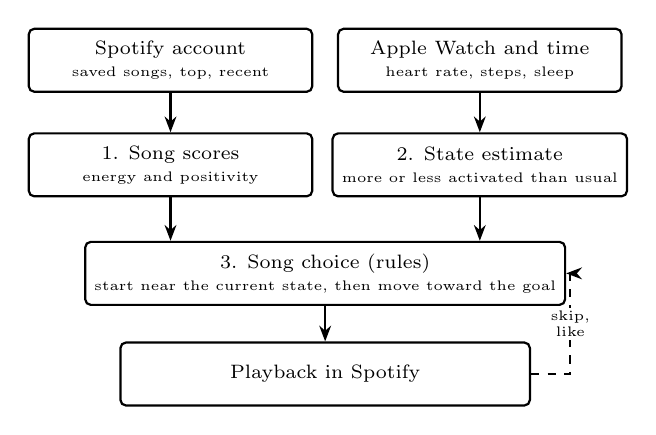
\begin{tikzpicture}[node distance=0.5cm]
\node[box, minimum width=3.6cm] (sp) {Spotify account\\{\tiny saved songs, top, recent}};
\node[box, minimum width=3.6cm, right=0.3cm of sp] (wt) {Apple Watch and time\\{\tiny heart rate, steps, sleep}};
\node[box, minimum width=3.6cm, below=of sp] (s1) {1. Song scores\\{\tiny energy and positivity}};
\node[box, minimum width=3.6cm, below=of wt] (s2) {2. State estimate\\{\tiny more or less activated than usual}};
\node[box, minimum width=5.2cm, below=0.55cm of $(s1.south)!0.5!(s2.south)$] (s3) {3. Song choice (rules)\\{\tiny start near the current state, then move toward the goal}};
\node[box, minimum width=5.2cm, below=0.45cm of s3] (pl) {Playback in Spotify};
\draw[flow] (sp) -- (s1);
\draw[flow] (wt) -- (s2);
\draw[flow] (s1.south) -- (s1.south |- s3.north);
\draw[flow] (s2.south) -- (s2.south |- s3.north);
\draw[flow] (s3) -- (pl);
\draw[flow, dashed] (pl.east) -- ++(0.5,0) |- node[lbl, pos=0.25]{skip,\\like} (s3.east);
\end{tikzpicture}
\caption{System overview. The dashed arrow is the feedback from the listener.}
\label{fig:overview}
\end{figure}

\textbf{Song scores.} Spotify removed its audio features (valence, energy) for new apps in November 2024~\cite{spotify2024}, so the app cannot analyse the sound. We use \textbf{MuSe}, a public dataset of 90,408 songs with valence and arousal scores built from Last.fm tags, with tentative Spotify IDs for about 68\% of them~\cite{muse}. For songs not in MuSe, a large language model (LLM) estimates the two scores from the title and artist; this estimate is checked on songs present in MuSe.

\textbf{State estimate.} A small model says whether the person is currently more or less activated than usual, never a named emotion. Asking each user for weeks of personal data would make a poor first day, so we train on \textbf{EmoPhone}~\cite{emophone}: three yearly waves (2020--2022) of university students in Korea who wore a Fitbit and answered short mood questions about seven times a day for four weeks (297 participants after quality control). Its \emph{arousal} answer, turned into ``above or below this person's own average'', is exactly our output. The model uses four inputs: the time of day, the heart rate, the steps and last night's sleep, each compared with the person's own average over the last 7 to 14 days, which needs no training on the user. A night or a period when the watch was not worn is marked as unknown, never as zero sleep or zero steps. The dataset authors granted us access for this project; the data files stay on team computers (NFR9).

\textbf{Song choice.} Rules build a queue of 3 to 5 songs: the first one or two match the current state, the next ones move step by step toward the goal of the situation. This follows the \textbf{iso principle} of music therapy, supported by a controlled experiment on mood after a sad film clip~\cite{iso}. If the library has too few suitable songs, at most two MuSe songs close to the user's taste complete the queue and are marked as new.

\textbf{An example.} At 11:30 p.m.\ the user taps Wind-down. The heart rate is above the person's usual evening value, so the first two songs have a medium energy and the next ones become calmer step by step. A skip is recorded for future queues.

\textbf{How we will test it.} (1) Song scores: correlation between the LLM estimate and MuSe on shared songs. (2) State estimate: tests on people the model has not seen, never a random split of one person's data, then on a whole held-out wave, compared with a time-of-day baseline; if the model does not beat the baseline, it is not used. (3) Pilot: at most five Spotify accounts (the limit of Spotify's development mode~\cite{spotify2026}) for about two weeks, comparing skip rates and a one-tap ``did this fit?'' answer between our queues and queues built from the time of day only. The pilot measures fit, not health benefits.

\textbf{Limits.} The app is a demonstrator for five users and a wellness companion, not a medical tool. The training data come from a Fitbit and Android phones, not from an Apple Watch, so the pilot measures the remaining gap. Accuracy is modest (Section~\ref{sec:req4}); the one-tap situation choice keeps the app useful when the estimate is wrong.

\textbf{Going further.} All music access goes through one small interface and all health data through another, so supporting Apple Music, Deezer or a watch on Android means writing one new connector (Section~\ref{sec:req7}).

\subsection{Development Plan (revised)}\label{sec:plan}
Each milestone ends with a demo to the customer. The plan of Submission~A put M1 at the end of October; the dates below replace it.
\begin{itemize}
\item \textbf{M1, Nov.\ 15:} Spotify sign-in and import tested with a live account, reading of Apple Health data, demo mode.
\item \textbf{M2, Nov.\ 29:} song scores; state model trained on EmoPhone and tested on held-out people and a held-out wave.
\item \textbf{M3, Dec.\ 6:} queue building, playback, feedback, explanation and data-control screens.
\item \textbf{M4, Dec.\ 7 to end of term:} pilot (about two weeks), evaluation, final report and demo.
\end{itemize}
All code goes through pull requests on GitHub, reviewed by another member; the team meets weekly and decides together.

\textbf{Changes since Submission A.} EmoPhone replaces UC Irvine and PMData as training data (larger, in-the-moment labels, Korean students). The model inputs are now the time of day, the heart rate, the steps and last night's sleep. Heart-rate variability is no longer a model input, because EmoPhone does not contain it; it is still read for the explanation. EmoPhone has no watch-measured sleep either, so for training we estimate it from the Fitbit heart rate and steps (Section~\ref{sec:req4}). The weather is removed: EmoPhone locations are anonymised, so weather cannot be matched to each participant. The plan has new dates, and NFR9 is new.

%=====================================================================
\section{Requirements}
%=====================================================================
Priorities: Must, Should, Could. Requirements keep their numbers from Submission~A and are grouped by module; ``(rev.)'' marks a change.

\subsection{Spotify Connection}
The app must connect to the user's Spotify account, read the library and play music.
\begin{itemize}
\item \textbf{FR1. Sign-in (Must):} connect through Spotify's secure sign-in (OAuth) and disconnect at any time.
\item \textbf{FR2. Library import (Must):} download all saved songs (title, artists, cover art), page by page, and store them on the phone.
\item \textbf{FR9. Playback (Must):} start the queue in Spotify; if this fails, open the songs in the Spotify app.
\item \textbf{NFR6. Spotify rules:} show cover art unaltered, the Spotify logo and a link to Spotify.
\end{itemize}

\subsection{Watch Data and Personal Average}
\begin{itemize}
\item \textbf{FR3. Watch data (Must, rev.):} with permission, read heart rate, heart-rate variability, sleep and steps from Apple Health when the app is opened. Heart rate, steps and sleep feed the model; heart-rate variability feeds the explanation.
\item \textbf{FR4. Personal average (Must):} compute the person's usual values over 7 to 14 days and compare recent values with them.
\item \textbf{NFR4. Missing data and watch not worn:} a night or a period without heart-rate samples is marked as unknown, never as zero sleep or zero steps; if watch data are missing or old, the app still works from the time of day and the library.
\end{itemize}

\subsection{Song Scores}
\begin{itemize}
\item \textbf{FR6. Song scores (Must):} give each song an energy and a positivity score from MuSe, or from an LLM estimate when it is not found (Should).
\end{itemize}

\subsection{State Estimate}
\begin{itemize}
\item \textbf{FR7. State estimate (Must, rev.):} estimate whether the person is more or less activated than usual with a model trained on EmoPhone.
\item \textbf{NFR7. Responsible use:} no medical claim, no emotion label shown to the user; the user can always stop or change the music.
\end{itemize}

\subsection{Situation and Queue}
\begin{itemize}
\item \textbf{FR5. Situation choice (Must):} four one-tap buttons (Table~\ref{tab:situations}), with one suggested from the time, the state and last night's sleep (Should).
\item \textbf{FR8. Queue building (Must):} 3 to 5 songs from the library, starting near the current state and moving toward the goal, with at most two matching songs; at most two MuSe songs when the library is not enough (Should).
\item \textbf{FR11. Explanation (Should):} a short reason, e.g. ``short night, morning: calm songs first, then more energy''.
\item \textbf{NFR3. Speed:} a queue within 2 s of the tap; 2,000 songs imported in under 60 s on Wi-Fi.
\item \textbf{NFR5. Ease of use:} at most two taps from launch to music.
\end{itemize}

\subsection{Feedback, Data Control and Security}
\begin{itemize}
\item \textbf{FR10. Feedback (Must):} record skips, likes and a ``did this fit?'' answer, and avoid disliked songs.
\item \textbf{FR13. Data control (Must):} view, export and delete all stored data.
\item \textbf{NFR1. Privacy:} health data stay on the phone; the LLM only receives titles and artists; explicit consent per data source.
\item \textbf{NFR2. Security:} Spotify tokens in the iOS Keychain; no API key inside the app; HTTPS only.
\end{itemize}

\subsection{Demo Mode, Tests and Other Services}
\begin{itemize}
\item \textbf{FR12. Demo mode (Should):} run the app on recorded data, without a live watch.
\item \textbf{NFR8. Testability:} song scores, state estimate and song choice covered by automated tests on recorded data.
\item \textbf{FR14. Other services (Could):} support another music service or watch through the same interfaces.
\end{itemize}

\subsection{Dataset Terms}
\begin{itemize}
\item \textbf{NFR9. Dataset terms (new):} EmoPhone data are used on team computers only, never committed to the public repository or shipped in the app.
\end{itemize}

%=====================================================================
\section{Development Environment}
%=====================================================================
\subsection{Choice of Software Development Platform}
The app is developed as a native \textbf{iOS application}. The Apple Watch data are only available on the iPhone through \textbf{HealthKit}, and the \textbf{Spotify iOS SDK}, which controls playback, also runs on the iPhone; a web app could read neither. Building an iPhone app requires \textbf{Xcode} on \textbf{macOS}, so the app is developed on a MacBook. The data and AI part is written in \textbf{Python} and runs on a Windows computer; only the final conversion to Core ML is done on the Mac. The trained model is converted to \textbf{Core ML} and runs on the phone, so no database server is needed: health data never leave the phone (NFR1). One small cloud part remains: the LLM API key must not be stored in the app, because anyone could extract it from the installed app. Song-score requests therefore go through a \textbf{Cloudflare Worker}, a serverless function that holds the key, accepts only titles and artists, and limits the number of requests per user. The free plan allows 100,000 requests per day~\cite{cfworkers}, far above our needs. Table~\ref{tab:tools} explains each choice.

\begin{table}[H]
\centering
\caption{Tools and Language Choice}
\label{tab:tools}
\scriptsize
\begin{tabularx}{\columnwidth}{|>{\raggedright\arraybackslash}p{1.85cm}|>{\raggedright\arraybackslash}X|}
\hline
\textbf{Tool / language} & \textbf{Reason} \\ \hline
\textbf{Swift + SwiftUI} & Apple's main language; HealthKit and Core ML are designed for it; SwiftUI builds screens with little code. \\ \hline
\textbf{HealthKit} & Only way to read Apple Watch heart rate, heart-rate variability, sleep and steps, with per-signal consent. \\ \hline
\textbf{Spotify Web API + iOS SDK} & Web API for the library and track lookup; iOS SDK to play and queue songs in the Spotify app. \\ \hline
\textbf{SwiftData} & Local storage on the phone for songs, scores, summaries and feedback, with no server. \\ \hline
\textbf{Python, pandas, scikit-learn} & Reading the dataset files; logistic regression and \texttt{GroupKFold} to test on people kept apart. \\ \hline
\textbf{coremltools + Core ML} & Converts the trained model so it runs on the phone, offline. \\ \hline
\textbf{LLM API (Claude Haiku 5.5)} & Scores songs missing from MuSe from title and artist, in batches, cached; low cost (final model chosen in the design phase). \\ \hline
\textbf{Cloudflare Workers} & Serverless proxy that keeps the LLM API key out of the app and limits requests; free plan, no server to maintain. \\ \hline
\textbf{GitHub + LaTeX} & Version control and pull-request reviews; documents in the IEEE template. \\ \hline
\end{tabularx}
\end{table}

\textbf{Development environment.} Table~\ref{tab:env} gives the machines and versions. scikit-learn is kept at version 1.5, the latest supported by coremltools 8 for model conversion~\cite{coremltools}.

\begin{table}[H]
\centering
\caption{Development Environment}
\label{tab:env}
\scriptsize
\begin{tabularx}{\columnwidth}{|>{\raggedright\arraybackslash}p{2.2cm}|>{\raggedright\arraybackslash}X|}
\hline
\textbf{Item} & \textbf{Version or resources} \\ \hline
Mac (app) & MacBook Air M3, 24 GB RAM; macOS 27.2 \\ \hline
Xcode, Swift & Xcode 27.2, Swift 6 language mode \\ \hline
App target & iOS 18.0 minimum (SwiftData, current HealthKit APIs) \\ \hline
iPhone, Apple Watch & iPhone 16 (iOS 27.2); Apple Watch Series 9 (watchOS 27.2) \\ \hline
Computer (data and AI) & Windows 11, 32 GB RAM \\ \hline
Python and libraries & Python 3.12; pandas 2.2, scikit-learn 1.5, coremltools 8.3 (model conversion run on the Mac) \\ \hline
Spotify iOS SDK & 5.0.1, through Swift Package Manager \\ \hline
Cloud & Cloudflare Workers (free plan), deployed with the Wrangler command-line tool \\ \hline
\end{tabularx}
\end{table}

\subsection{Cost Estimation}
The team uses Macs, iPhones and watches it already owns, and all development tools are free (Xcode, Python, GitHub, LaTeX). Four costs remain (Table~\ref{tab:cost}). The \textbf{Apple Developer Program} costs US\$99 per year~\cite{appledev}; one membership is enough for the team, and without it an app installed from Xcode expires after 7 days~\cite{applemember}. \textbf{Spotify Premium} is required for the app owner in development mode and for playback~\cite{spotify2026}; members already subscribed pay nothing extra~\cite{spotifykr}. The \textbf{LLM} cost is negligible: about 6,000 songs (four libraries plus the check on MuSe) at about 200 tokens each, at the batch price of Claude Haiku 5.5~\cite{claudeprice}, is under US\$1. The team also uses AI assistants to help with development: four \textbf{Claude Pro} subscriptions at US\$20 per month~\cite{claudepro} for the two months of the project, US\$160 in total. The Cloudflare Worker stays within the free plan~\cite{cfworkers}.

\begin{table}[H]
\centering
\caption{Cost Estimation (prices checked Nov.\ 4, 2026)}
\label{tab:cost}
\scriptsize
\begin{tabularx}{\columnwidth}{|>{\raggedright\arraybackslash}X|>{\raggedright\arraybackslash}p{3.2cm}|}
\hline
\textbf{Item} & \textbf{Cost} \\ \hline
Apple Developer Program (one for the team) & US\$99 per year \\ \hline
Spotify Premium, per account not yet subscribed & KRW 11,990 / month (KRW 6,600 student) \\ \hline
LLM song scores & under US\$1 in total \\ \hline
Claude Pro for development (4 members, 2 months) & 4 $\times$ 2 $\times$ US\$20 = US\$160 \\ \hline
Cloudflare Workers (LLM proxy) & free plan \\ \hline
Hardware and software tools & already owned or free \\ \hline
\end{tabularx}
\end{table}

\subsection{Software in Use}
\subsubsection{Existing Systems / Tools}
\textbf{Endel}~\cite{endel} adapts generated soundscapes to heart rate, time and weather. It shows that body signals are useful for music, but it does not play the user's own songs.

\textbf{Spotify daylist and Prompted Playlists}~\cite{daylist},~\cite{prompted} personalise playlists from listening history, time of day or a typed prompt. They play the user's music but ignore the body.

\textbf{MuSe}~\cite{muse} gives valence and arousal for 90,408 songs (CC~BY~4.0). We use it directly as song scores.

\textbf{EmoPhone and its benchmark}~\cite{emophone} provide the training data and an evaluation method: features from the minutes before each mood answer, normalisation per person, and labels relative to each person's average. On people not seen in training, its best models reach an AUROC of about 0.58 for arousal with thousands of phone and watch features (0.5 is chance).

\textbf{WatchAnxiety}~\cite{watchanxiety} predicts a yes/no anxiety state from smartwatch heart rate and reports 60.4\% balanced accuracy, another sign that realistic results are modest.

\subsubsection{Comparison \& Gap Analysis}
\begin{itemize}
\item \textbf{Body and own music:} Endel uses the body but not the user's songs; Spotify uses the user's songs but not the body. Our app combines both.
\item \textbf{Clear goal:} existing playlists follow the user's habits; our queue has a goal (calmer or more energetic) and a path toward it.
\item \textbf{Transparency:} simple rules and a small model, so each queue can be explained to the user (FR11) and tested.
\item \textbf{Privacy:} the model runs on the phone; health data are never sent to a server, only song titles to the LLM proxy.
\end{itemize}

\subsection{Task Distribution}
The detailed task distribution will be given in the design phase, once the modules and their interfaces are fixed. Until then, the work follows the roles of Table~\ref{tab:roles}.

%=====================================================================
\section{Specifications}\label{sec:spec}
%=====================================================================
Each requirement group of Section~III is described with its goal, implementation and pseudo-code. This section is a plan: the code is written in the next phases.

\subsection{Requirement 1 -- Spotify Connection (FR1, FR2, FR9, NFR6)}
\goal{Connect the user's Spotify account, import the library and play a queue.}
\impl
\begin{itemize}
\item \textbf{App:} ``Connect Spotify'' screen; OAuth with PKCE, so no client secret is stored in the app; tokens in the Keychain (NFR2).
\item \textbf{Spotify Web API:} the February 2026 changes keep the endpoints we need: \texttt{GET /me/tracks}, \texttt{/me/top/tracks}, \texttt{/me/player/recently-played} and \texttt{GET /tracks/\{id\}}. The batch lookup \texttt{GET /tracks} was removed, and saving a song now uses \texttt{PUT /me/library}~\cite{spotify2026}. Each call is checked with a live account in M1.
\item \textbf{Playback:} Spotify iOS SDK plays the first song and adds the others to the Spotify queue; if the SDK cannot connect, the song opens in the Spotify app.
\item \textbf{Screen:} cover art unaltered, Spotify logo and link (NFR6).
\end{itemize}
\par\noindent\begin{minipage}{\columnwidth}
\pcode
\begin{code}
connectSpotify():                  # OAuth with PKCE
  code   = openSpotifyLogin(sha256(verifier))
  tokens = exchange(code, verifier) -> Keychain
importLibrary():
  url = "/me/tracks?limit=50"
  while url:
    page = GET(url)                  # retry on 429
    db.tracks.upsert(page.items); url = page.next
  add top tracks and recent plays; score new songs
\end{code}
\end{minipage}\par

\subsection{Requirement 2 -- Watch Data and Personal Average (FR3, FR4, NFR4)}
\goal{Read the watch data and compare recent values with the person's own usual values.}
\impl
\begin{itemize}
\item \textbf{HealthKit:} anchored queries on opening (Apple Health cannot be read while the phone is locked); one consent per signal.
\item \textbf{Summaries:} raw samples are turned into hourly and nightly summaries, then dropped (NFR1).
\item \textbf{Personal average:} mean and standard deviation per 3-hour block of the day over the last 14 days, ready after 7 days; heart rate depends strongly on the time of day.
\item \textbf{Sleep:} HealthKit sleep samples recorded by the Apple Watch only; ``in bed'' periods set on the iPhone are ignored.
\item \textbf{Watch worn?} The watch measures heart rate only when it is on the wrist, so a night counts only if heart-rate samples cover at least 60\% of the 21:00--12:00 window; otherwise last night's sleep is \emph{unknown}, not zero. The same rule applies to steps in the last 30 minutes (NFR4).
\item \textbf{Missing data:} an unknown value is replaced by the person's usual value and flagged for the model; without heart rate in the last 30 minutes, the app falls back on the time of day.
\end{itemize}
\par\noindent\begin{minipage}{\columnwidth}
\pcode
\begin{code}
onAppOpen():
  for s in [heartRate, hrv, sleep, steps] if consent(s):
    samples = HealthKit.query(s, after=anchor[s])
    db.summaries.update(hourly(samples))
  night = last 21:00-12:00 window
  worn  = share of minutes with heart rate in night
  sleep = watchSleep(night) if worn >= 0.6 else UNKNOWN
  for s, block in signals x 3-hour blocks:
    v = summaries(s, block, last 14 days)
    baseline[s, block] = (mean(v), sd(v)) if days(v) >= 7
                         else NONE
\end{code}
\end{minipage}\par

\subsection{Requirement 3 -- Song Scores (FR6)}
\goal{Give every library song an energy and a positivity score between 0 and 1.}
\impl
\begin{itemize}
\item \textbf{MuSe table:} shipped with the app (title, artists, scores, Spotify ID), rescaled to 0--1; matched by Spotify ID, then by normalised title and artist.
\item \textbf{LLM:} songs still missing are sent in batches of 50 (titles and artists only) to the Cloudflare Worker, which adds the API key and calls the LLM; the JSON answer is checked and cached, so each song is sent once.
\item \textbf{Check:} offline, the same prompt is run on 2,000 MuSe songs; we report the correlation and the mean error.
\end{itemize}
\par\noindent\begin{minipage}{\columnwidth}
\pcode
\begin{code}
for t in tracks without score:
  m = muse.byId(t.id) or muse.byTitleArtist(norm(t))
  if m: save(t, m.arousal, m.valence, origin="MuSe")
  else: missing.append(t)
for batch in chunks(missing, 50):
  scores = POST worker/score {titlesAndArtists(batch)}
  save(batch, valid(scores) or 0.5, origin="LLM")
\end{code}
\end{minipage}\par

\subsection{Requirement 4 -- State Estimate (FR7, NFR7)}\label{sec:req4}
\goal{Estimate, between 0 and 1, whether the person is more or less activated than usual.}
\impl
\begin{itemize}
\item \textbf{Training data:} EmoPhone. For each mood answer: the heart rate and the steps in the 15, 30 and 60 minutes before it, last night's sleep duration and the time since waking up, all compared with the person's own average, plus the hour of the day. The label is 1 when the arousal answer is above the person's own average.
\item \textbf{Sleep in training:} EmoPhone has no watch-measured sleep, so we estimate it the way watches do: the longest period between 21:00 and 12:00 with the watch worn, no steps and a heart rate in the person's lowest 30\%, lasting at least 2 hours. The median is 7.3 hours. The watch was not worn on 34\% of nights; those nights are marked unknown, as in the app.
\item \textbf{Model:} logistic regression (scikit-learn), tested with a 5-fold split by participant; kept only if it beats the time-of-day baseline; converted with coremltools.
\item \textbf{On the phone:} the same features come from Requirement~2; Core ML returns a number, never an emotion label (NFR7).
\end{itemize}

\par\noindent\begin{minipage}{\columnwidth}
\pcode
\begin{code}
# offline, Python
x = [z(HR_15), z(HR_30), z(HR_60), z_block(HR_30),
     z(steps_15), z(steps_30), z(steps_60),
     z(sleep), hoursSinceWake, sleepUnknown,
     sin(hour), cos(hour), weekend]
y = arousal > mean arousal of this participant
for fold in GroupKFold(5, groups=participant):
  fit LogisticRegression; report AUROC, balanced accuracy
keep if AUROC > time-only baseline -> StateModel.mlmodel

# on the phone
if no baseline or no heart rate in last 30 min:
  return prior(hour)             # time-of-day mode
# 0 = calmer than usual .. 1 = more activated
return StateModel.predict(x)
\end{code}
\end{minipage}\par

\textbf{First results.} We ran this pipeline on the first EmoPhone wave (92 participants, 10,259 answers); Table~\ref{tab:results} gives the results. Our four-input model reaches an AUROC of 0.573, the level of the best published models on this wave, which use thousands of phone and watch features~\cite{emophone}. Heart rate carries most of the information. On this wave, steps and sleep do not add a measurable gain: the four-input model is within the variation between folds ($\pm$0.015) of the heart-rate model. We keep them because the Apple Watch measures sleep itself, whereas EmoPhone sleep had to be estimated, and because they drive the rules. The held-out waves and the pilot will show whether they help; if not, the app uses the heart-rate model. The result is unchanged with one heart-rate reading every 5 minutes, which matters because the Apple Watch is expected to measure less often than the Fitbit. Stress is barely predictable, so the Stress situation is chosen by the user. The mood of the \emph{other} participants at the same date and time, which includes shared effects such as the weather, gives only 0.53, so removing the weather costs little. These are first results on one wave.

\begin{table}[H]
\centering
\caption{First Results on EmoPhone Wave 1 (people kept apart)}
\label{tab:results}
\scriptsize
\begin{tabularx}{\columnwidth}{|>{\raggedright\arraybackslash}X|>{\raggedright\arraybackslash}p{1.0cm}|>{\raggedright\arraybackslash}p{1.0cm}|}
\hline
\textbf{Target and inputs} & \textbf{AUROC} & \textbf{Bal.\ acc.} \\ \hline
Arousal: time of day only & 0.532 & 0.509 \\ \hline
Arousal: time + sleep & 0.526 & 0.507 \\ \hline
Arousal: time + heart rate & 0.577 & 0.547 \\ \hline
Arousal: time + heart rate + steps & 0.577 & 0.547 \\ \hline
\textbf{Arousal: time + heart rate + steps + sleep (our model)} & \textbf{0.573} & \textbf{0.542} \\ \hline
Arousal: same, gradient-boosted trees & 0.558 & 0.533 \\ \hline
Arousal: time + heart rate, one reading every 5 min & 0.575 & -- \\ \hline
Stress: our model & 0.543 & 0.514 \\ \hline
Arousal: other participants at same date and time & 0.530 & -- \\ \hline
\end{tabularx}
\end{table}



\subsection{Requirement 5 -- Situation and Queue (FR5, FR8, FR11, NFR3, NFR5)}
\goal{Suggest a situation and build a short queue that goes from the current state to the goal.}
\impl
\begin{itemize}
\item \textbf{Home screen:} four large buttons; the suggested one is highlighted: wake-up within two hours after the end of sleep, wind-down after 21:00, low energy between 13:00 and 17:00 when the state is below 0.4.
\item \textbf{Queue rules:} target energies go from the state to the goal of the situation (e.g.\ 0.2 for wind-down, 0.7 for wake-up); for each position, the closest library song is chosen, preferring positive songs for stress and low energy, avoiding repeated artists and songs played in the last 3 days.
\item \textbf{MuSe fallback:} when no library song is within 0.15 of the target, a MuSe song with a shared artist or genre is checked with \texttt{GET /tracks/\{id\}} and marked as new (at most two).
\item \textbf{Explanation:} built from fixed sentence parts, e.g.\ ``heart rate higher than usual: medium songs first, then calmer''.
\item \textbf{Speed:} the queue is built from local data, with at most a few lookups (NFR3).
\end{itemize}
\par\noindent\begin{minipage}{\columnwidth}
\pcode
\begin{code}
buildQueue(situation, e0):     # e0 = state estimate
  g = goal[situation]
  n = 5 if |e0 - g| > 0.3 else 3
  m = 2 if n == 5 else 1       # matching songs
  targets = [e0]*m + evenly(e0 -> g, n - m)
  for e in targets:
    c = closest library song to e
        (not recent, not skipped, with penalties)
    if |energy(c) - e| > 0.15 and suggestions < 2:
      c = museSuggestion(e)    # checked on Spotify
    queue.add(c)
  return queue, explain(context, plan)
\end{code}
\end{minipage}\par

\subsection{Requirement 6 -- Feedback, Data Control and Security (FR10, FR13, NFR1, NFR2)}
\goal{Learn from skips and likes, and give the user full control over the stored data.}
\impl
\begin{itemize}
\item \textbf{Player screen:} skip, like and, after the queue, ``did this fit?''. A song skipped twice in a situation is left out of it; a skipped suggestion is never proposed again; a like saves the song to the library.
\item \textbf{Settings screen:} lists the stored data and consents; export as one JSON file; delete everything after a confirmation.
\item \textbf{Security:} tokens in the Keychain, HTTPS only (App Transport Security on); the LLM key stays in the Cloudflare Worker, and the request contains titles and artists only.
\end{itemize}
\par\noindent\begin{minipage}{\columnwidth}
\pcode
\begin{code}
on skip (before 30 s): save(skip)
on like:               save(like); PUT /me/library
after last song:       ask "Did this fit?"
deleteAll():
  clear tracks, scores, summaries, queues,
        feedback, consents
  Keychain.delete(tokens); reset HealthKit anchors
\end{code}
\end{minipage}\par

\subsection{Requirement 7 -- Demo Mode, Tests and Other Services (FR12, FR14, NFR8)}\label{sec:req7}
\goal{Run and test the app without a live watch, and keep Spotify and Apple Health replaceable.}
\impl
\begin{itemize}
\item \textbf{Interfaces:} the song scores, state estimate and queue rules only see two Swift protocols. A new service (Apple Music, Deezer, Health Connect on Android) means one new implementation.
\item \textbf{Demo mode:} both protocols implemented with recorded files (a few days of a team member's summaries, a small song list); no EmoPhone data (NFR9).
\item \textbf{Tests:} XCTest unit tests on these files (z-scores, baselines, queue rules such as ``never more than two suggestions'', LLM answer parser); pytest for the Python code.
\end{itemize}
\par\noindent\begin{minipage}{\columnwidth}
\begin{code}
protocol MusicProvider {
  func signIn() async throws
  func importLibrary() async throws -> [Track]
  func play(_ q: Queue) async throws
  func save(_ t: Track) async throws
}
protocol HealthProvider {
  func requestConsent(_ s: Set<Signal>) async
  func newSamples(_ s: Signal) async -> [Sample]
}
\end{code}
\end{minipage}\par

\subsection{Requirement 8 -- Data Storage and Dataset Terms (NFR1, NFR9)}
\goal{Store all app data on the phone, and keep the training data out of the public repository.}
\impl
\begin{itemize}
\item \textbf{Phone:} SwiftData tables below; the MuSe table and the Core ML model are read-only files in the app; tokens in the Keychain.
\item \textbf{Repository:} \texttt{data/} is listed in \texttt{.gitignore}, and the repository is checked before each submission (NFR9).
\end{itemize}
\par\noindent\begin{minipage}{\columnwidth}
\textbf{Schema:}
\begin{code}
tracks:    { spotifyId, title, artists[], coverURL,
             source, addedAt }
scores:    { spotifyId, energy, positivity, origin }
hours:     { hourStart, meanHR, sdnnHRV, steps }
nights:    { date, sleepMinutes, sleepEnd, worn }
baselines: { signal, block3h, mean, sd, nDays }
queues:    { id, situation, startEnergy, kind,
             reason, items[] }
feedback:  { queueId, spotifyId, event, seconds, time }
consents:  { source, granted, time }
Keychain:  { accessToken, refreshToken, expiresAt }
\end{code}
\end{minipage}\par

\subsection{System Integration Workflow}
\par\noindent\begin{minipage}{\columnwidth}
\textbf{Data flow:}
\begin{code}
[Apple Health] -> Health connector -> hours, baselines
                                          |
[Spotify] -> Music connector -> tracks -> Song scores
                     (MuSe / LLM via Cloudflare Worker)
                                          |
user taps a situation -> State model (Core ML)
                                          |
                     Queue rules + explanation
                                          |
[Spotify app] <- play / queue     skip, like -> feedback
\end{code}
\end{minipage}\par

%=====================================================================
\enlargethispage{3\baselineskip}
\begin{thebibliography}{99}
\setlength{\itemsep}{0pt}
\footnotesize
\bibitem{koreatimes_sleep} Y. Whan-woo, ``Sleep market in Korea reaches W3 tril. says report,'' \textit{The Korea Times}, Apr.\ 10, 2024. [Online]. Available: \url{https://www.koreatimes.co.kr/www/biz/2024/04/126_372435.html}
\bibitem{cochrane} K. V. Jespersen, V. Pando-Naude, J. Koenig, P. Jennum, and P. Vuust, ``Listening to music for insomnia in adults,'' \textit{Cochrane Database Syst. Rev.}, no.~8, Art.\ no.\ CD010459, 2022, doi: 10.1002/14651858.CD010459.pub3.
\bibitem{endel} Endel, ``Endel: personalized soundscapes.'' [Online]. Available: \url{https://endel.io/} (accessed Oct.\ 20, 2026).
\bibitem{daylist} ``Spotify launches ever-changing `Daylist' playlist that adapts to users' moods,'' \textit{Music Business Worldwide}, 2023. [Online]. Available: \url{https://musicbusinessworldwide.com/spotify-launches-ever-changing-daylist-playlist-that-adapts-to-users-moods}
\bibitem{prompted} ``Spotify brings AI-powered Prompted Playlists to the U.S. and Canada,'' \textit{TechCrunch}, Jan.\ 22, 2026. [Online]. Available: \url{https://techcrunch.com/2026/01/22/spotify-brings-ai-powered-prompted-playlists-to-the-u-s-and-canada/}
\bibitem{lozano} \'A. Lozano Murciego, D. M. Jim\'enez-Bravo, A. Valera Rom\'an, J. F. De Paz Santana, and M. N. Moreno-Garc\'ia, ``Context-aware recommender systems in the music domain: a systematic literature review,'' \textit{Electronics}, vol.~10, no.~13, Art.\ no.\ 1555, 2021.
\bibitem{spotify2024} Spotify for Developers, ``Introducing some changes to our Web API,'' Nov.\ 27, 2024. [Online]. Available: \url{https://developer.spotify.com/blog/2024-11-27-changes-to-the-web-api}
\bibitem{muse} C. Akiki and M. Burghardt, ``MuSe: The Musical Sentiment Dataset,'' \textit{J. Open Humanit. Data}, vol.~7, 2021, doi: 10.5334/johd.33.
\bibitem{emophone} P. Zhang, M. Park, S. Kang \textit{et al.}, ``EmoPhone: A multi-wave dataset for in-the-wild mobile and wearable affect sensing,'' arXiv:2609.16581, 2026. Data: Harvard Dataverse, doi: 10.7910/DVN/QGRVU8.
\bibitem{iso} K. Starcke, J. Mayr, and R. von Georgi, ``Emotion modulation through music after sadness induction---the iso principle in a controlled experimental study,'' \textit{Int. J. Environ. Res. Public Health}, vol.~18, no.~23, Art.\ no.\ 12486, 2021.
\bibitem{spotify2026} Spotify for Developers, ``Web API changes, February 2026'' and ``February 2026 dev mode changes: migration guide.'' [Online]. Available: \url{https://developer.spotify.com/documentation/web-api/references/changes/february-2026} (accessed Nov.\ 4, 2026).
\bibitem{watchanxiety} M. S. Ahmed \textit{et al.}, ``WatchAnxiety: a transfer learning approach for state anxiety prediction from smartwatch data,'' arXiv:2509.13725, 2025.
\bibitem{appledev} Apple, ``Apple Developer Program.'' [Online]. Available: \url{https://developer.apple.com/programs/} (accessed Nov.\ 4, 2026).
\bibitem{applemember} Apple, ``Choosing a membership.'' [Online]. Available: \url{https://developer.apple.com/support/compare-memberships} (accessed Nov.\ 4, 2026).
\bibitem{spotifykr} Spotify, ``Premium plans (Korea).'' [Online]. Available: \url{https://www.spotify.com/kr-en/premium} (accessed Nov.\ 4, 2026).
\bibitem{coremltools} Apple, ``coremltools releases.'' [Online]. Available: \url{https://github.com/apple/coremltools/releases} (accessed Nov.\ 4, 2026).
\bibitem{claudepro} Anthropic, ``Plans \& pricing.'' [Online]. Available: \url{https://claude.com/pricing} (accessed Nov.\ 4, 2026).
\bibitem{cfworkers} Cloudflare, ``Limits,'' Cloudflare Workers docs. [Online]. Available: \url{https://developers.cloudflare.com/workers/platform/limits/} (accessed Nov.\ 4, 2026).
\bibitem{claudeprice} Anthropic, ``Pricing,'' Claude Platform Docs. [Online]. Available: \url{https://platform.claude.com/docs/en/about-claude/pricing} (accessed Nov.\ 4, 2026).
\end{thebibliography}

\end{document}
